\documentclass[12pt]{article}
\usepackage[english]{babel}
\usepackage[utf8]{inputenc}

%% Pointer to 'default' preamble
% pacakages and definitions

\usepackage{geometry}
\geometry{
	letterpaper, 
	portrait, 
	top=.75in,
	left=.8in,
	right=.75in,
	bottom=.5in		} 	% Page Margins
	
%% additional packages for nice things
\usepackage{amsmath} 	% for most math
\usepackage{commath} 	% for abs
\usepackage{lastpage}	% for page count
\usepackage{amssymb} 	% for therefore
\usepackage{graphicx} 	% for image handling
\usepackage{wrapfig} 	% wrap figures
\usepackage[none]{hyphenat} % for no hyphenations
\usepackage{array} 		% for >{} column characterisctis
\usepackage{physics} 	% for easier derivative \dv....
\usepackage{tikz} 		% for graphic@!
\usepackage{circuitikz} % for circuits!
\usetikzlibrary{arrows.meta} % for loads
\usepackage[thicklines]{cancel}	% for cancels
\usepackage{xcolor}		% for color cancels
\usepackage[per-mode=fraction]{siunitx} % for si units and num
\sisetup{group-separator = {,}, group-minimum-digits = 3} % additional si unit table functionality

\usepackage{fancyhdr} 	% for header
\usepackage{comment}	% for ability to comment out large sections
\usepackage{multicol}	% for multiple columns using multicols
\usepackage[framed,numbered]{matlab-prettifier} % matlab sytle listing
\usepackage{marvosym} 	% for boltsymbol lightning
\usepackage{pdflscape} 	% for various landscape pages in portrait docs.
%\usepackage{float}
\usepackage{fancyvrb}	% for Verbatim (a tab respecting verbatim)
\usepackage{enumitem}	% for [resume] functionality of enumerate
\usepackage{spreadtab} 	% for using formulas in tables}
\usepackage{numprint}	% for number format in spread tab
\usepackage{subcaption} % for subfigures with captions
\usepackage[normalem]{ulem} % for strike through sout

% for row colors in tables....
\usepackage{color, colortbl}
\definecolor{G1}{gray}{0.9}
\definecolor{G2}{rgb}{1,0.88,1}%{gray}{0.6}
\definecolor{G3}{rgb}{0.88,1,1}

% For table formatting
\usepackage{booktabs}
\renewcommand{\arraystretch}{1.2}
\usepackage{floatrow}
\floatsetup[table]{capposition=top} % put table captions on top of tables

% Caption formating footnotesize ~ 10 pt in a 12 pt document
\usepackage[font={small}]{caption}

%% package config 
\sisetup{output-exponent-marker=\ensuremath{\mathrm{E}}} % for engineer E
\renewcommand{\CancelColor}{\color{red}}	% for color cancels
\lstset{aboveskip=2pt,belowskip=2pt} % for more compact table
%\arraycolsep=1.4pt\def
\setlength{\parindent}{0cm} % Remove indentation from paragraphs
\setlength{\columnsep}{0.5cm}
\lstset{
	style      = Matlab-editor,
	basicstyle = \ttfamily\footnotesize, % if you want to use Courier - not really used?
}
\renewcommand*{\pd}[3][]{\ensuremath{\dfrac{\partial^{#1} #2}{\partial #3}}} % for larger pd fracs
\renewcommand{\real}[1]{\mathbb{R}\left\{ #1 \right\}}	% for REAL symbol
\newcommand{\imag}[1]{\mathbb{I}\left\{ #1 \right\}}	% for IMAG symbol
\definecolor{m}{rgb}{1,0,1}	% for MATLAB matching magenta
	
%% custom macros
\newcommand\numberthis{\addtocounter{equation}{1}\tag{\theequation}} % for simple \numberthis command

\newcommand{\equal}{=} % so circuitikz can have an = in the labels
\newcolumntype{L}[1]{>{\raggedright\let\newline\\\arraybackslash\hspace{0pt}}m{#1}}
\newcolumntype{C}[1]{>{\centering\let\newline\\\arraybackslash\hspace{0pt}}m{#1}}
\newcolumntype{R}[1]{>{\raggedleft\let\newline\\\arraybackslash\hspace{0pt}}m{#1}}

%% Header
\pagestyle{fancy} % for header stuffs
\fancyhf{}
% spacing
\headheight 29 pt
\headsep 6 pt

%% Header
\rhead{Thad Haines \\ Page \thepage\ of \pageref{LastPage}}
\chead{PST and VTS \\ - DRAFT -}
\lhead{Research \\ 08/04/20}
\usepackage{minted}
\usepackage{setspace}
\begin{document}
\onehalfspacing
\paragraph{Purpose} \ \\
This document is meant to explain PST additions and alterations created to accommodate VTS (variable time stepping).
While the current method works, it may change in the future.

\paragraph{Solution Control Array} \ \\
Between each \verb|sw_con| entry, a \emph{time block} is created that is then solved using a user defined solution method.
As such, the \verb|solver_con| array has 1 less row than the \verb|sw_con| array.
An example \verb|solver_con| array is shown below.
\begin{minted}[
		frame=lines,
		framesep=2mm,
		baselinestretch=1.2,
		bgcolor=gray!13,
		fontsize=\footnotesize,
		%linenos,
		breaklines
		]{MATLAB}
%% solver_con format
% A cell with a solver method in each row corresponding to the specified
% 'time blocks' defined in sw_con
%
% Valid solver names:
% huens - Fixed time step default to PST
% ode113 - works well during transients, consistent # of slns, time step stays relatively small
% ode15s - large number of slns during init, time step increases to reasonable size
% ode23 - realtively consisten # of required slns, timstep doesn't get very large
% ode23s - many iterations per step - not efficient...
% ode23t - occasionally hundereds of iterations, sometimes not... decent
% ode23tb - similar to 23t, sometimes more large solution counts

solver_con ={ ...
    'huens'; % pre fault - fault
    'huens'; % fault - post fault 1
    'huens'; % post fault 1 - post fault 2
    'huens'; % post fault 2 - sw_con row 5
    'huens'; % sw_con row 5 - sw_con row 6 
    'ode23t'; % sw_con row 6  - sw_con row 7  (end)
    };
\end{minted}

As of this writing, the pstSETO version uses the \verb|s_simu_BatchVTS| script to perform variable time stepping methods.
This script will likely replace the \verb|s_simu| script in the main PST4 folder after versioning is complete.\\

Theoretically, a user would only have to add a \verb|solver_con| to a data file to use variable time step methods.
If one is not specified, Huen's method is used for all time blocks (i.e. default PST behavior).


\pagebreak
\paragraph{MATLAB ODE solver} \ \\
The variable time step implementation in PST revolves around using the built in MATLAB ODE solvers.
All these methods perform actions depicted in the following block diagram.

\begin{center}
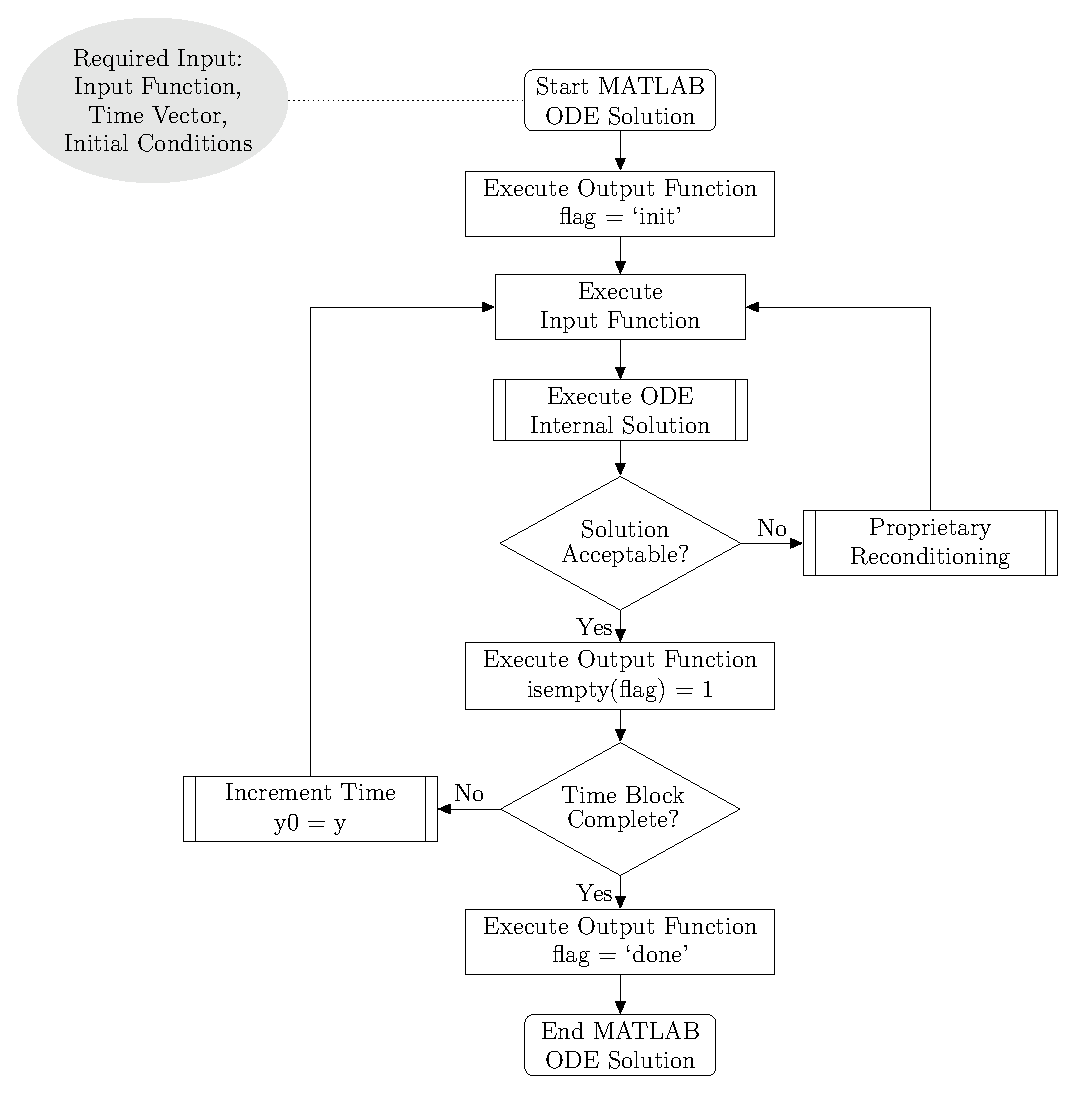
\includegraphics[width=.8\linewidth]{./../200804-ODEblockDiagram/200804-ODEblockDiagram}
\end{center}

The input to an ODE solver include, an input function, a time interval (time block), initial conditions, and solver options.
The current options used for VTS are shown below and deal with error tolerance levels, initial step size, max step size, and an Output function.

\begin{minted}[
		frame=lines,
		framesep=2mm,
		baselinestretch=1.2,
		bgcolor=gray!13,
		fontsize=\footnotesize,
	%	linenos,
		breaklines
				]{MATLAB}
% Configure ODE settings
%options = odeset('RelTol',1e-3,'AbsTol',1e-6); % default settings
options = odeset('RelTol',1e-3,'AbsTol',1e-6, ...
    'InitialStep', 1/60/4, ...
    'MaxStep',60, ...
    'OutputFcn',outputFcn); % set 'OutputFcn' to function handle
\end{minted}

\pagebreak
\paragraph{vtsInputFcn} \ \\
The slightly abbreviated input function is shown below.
\begin{minted}[
		frame=lines,
		framesep=2mm,
		baselinestretch=1.2,
		bgcolor=gray!13,
		fontsize=\footnotesize,
	%	linenos,
		breaklines
				]{MATLAB}
function [dxVec] = vtsInputFcn(t, y)
% VTSINPUTFCN passed to ODE solver to perfrom required step operations
%
%   NOTES: Updates g.vts.dxVec, and returns values
%
%   Input:
%   t - simulation time
%   y - solution vector (initial conditions)
%
%   Output:
%   dxVec - requried derivative vector for ODE solver

global g

%% call handleStDx with flag==2 to update global states with newest passed in soln.
% write slnVec vector of values to associated states at index k
% i.e. update states at g.vts.dataN with newest solution
handleStDx(g.vts.dataN, y, 2)

%% Start initStep action ==================================================
initStep(g.vts.dataN)

%% Start of Network Solution ==============================================
networkSolutionVTS(g.vts.dataN, t)

%% Start Dynamic Solution =================================================
dynamicSolution(g.vts.dataN )

%% Start of DC solution ===================================================
dcSolution(g.vts.dataN )

%% call handleStDx with flag==1 to update global dxVec
handleStDx(g.vts.dataN , [], 1) % update g.vts.dxVec (solution vector not needed)

dxVec = g.vts.dxVec; % return for ODE fcn requirements

if g.vts.iter == 0
    % save initial network solution
    handleNetworkSln(g.vts.dataN ,1)
end

g.vts.iter = g.vts.iter + 1; % increment iteration number
end % end vtsInputFcn
\end{minted}

\pagebreak

\paragraph{vtsOutputFcn} \ \\
The slightly abbreviated output function is shown below.
\begin{minted}[
		frame=lines,
		framesep=2mm,
		baselinestretch=1.2,
		bgcolor=gray!13,
		fontsize=\footnotesize,
	%	linenos,
		breaklines
				]{MATLAB}
function status = vtsOutputFcn(t,y,flag)
% VTSOUTPUTFCN performs associated flag actions with ODE solvers.
%
%   Input:
%   t - simulation time
%   y - solution vector
%   flag - dictate function action
%
%   Output:
%   status - required for normal operation (return 1 to stop)

global g 
status = 0; % required for normal operation

if isempty(flag) % normal step completion
    % restore network to initial solution
    handleNetworkSln(g.vts.dataN ,2) % may cause issues with DC.
    
    monitorSolution(g.vts.dataN); % Perform Line Monitoring and Area Calculations 
    
    %% Live plot call
    if g.sys.livePlotFlag
        livePlot(g.vts.dataN)
    end
    
    % after each successful integration step by ODE solver:
    g.vts.dataN = g.vts.dataN+1;    % increment logged data index 'dataN'
    g.sys.t(g.vts.dataN) = t;       % log step time
    g.vts.stVec = y;                % update state vector
    handleStDx(g.vts.dataN, y, 2)   % place new solution results into associated globals
    
    g.vts.tot_iter = g.vts.tot_iter + g.vts.iter;   % update total iterations
    g.vts.slns(g.vts.dataN) = g.vts.iter;           % log solution step iterations
    g.vts.iter = 0;                                 % reset iteration counter
    
elseif flag(1) == 'i' 
    % init solver for new time block
    g.sys.t(g.vts.dataN) = t(1);    % log step time
    handleStDx(g.vts.dataN, y, 2)   % log initial conditions
  
elseif flag(1) == 'd'
    % only debug screen output at the moment
end % end if
end % end function
\end{minted}

\pagebreak
\paragraph{Simulation Loop}
The complete simulation loop code is shown below.
This code was copied from \verb|s_simu_BatchVTS| with corresponding line numbers.

\begin{minted}[
		frame=lines,
		framesep=2mm,
		baselinestretch=1.2,
		bgcolor=gray!13,
		fontsize=\footnotesize,
		linenos,
		firstnumber=362,
		breaklines
				]{MATLAB}
%% Simulation loop start
warning('*** Simulation Loop Start')
for simTblock = 1:size(g.vts.t_block)
    
    g.vts.t_blockN = simTblock;
    g.k.ks = simTblock; % required for huen's solution method.
    
    if ~isempty(g.vts.solver_con)
        odeName = g.vts.solver_con{g.vts.t_blockN};
    else
        odeName = 'huens'; % default PST solver
    end
    
    if strcmp( odeName, 'huens')
        % use standard PST huens method
        fprintf('*** Using Huen''s integration method for time block %d\n*** t=[%7.4f, %7.4f]\n', ...
            g.vts.t_blockN, ...
            g.vts.fts{g.vts.t_blockN}(1), g.vts.fts{g.vts.t_blockN}(end))
        
        % add fixed time vector to system time vector
        nSteps = length(g.vts.fts{g.vts.t_blockN});
        g.sys.t(g.vts.dataN:g.vts.dataN+nSteps-1) = g.vts.fts{g.vts.t_blockN};
        
        % account for pretictor last step time check
        g.sys.t(g.vts.dataN+nSteps) = g.sys.t(g.vts.dataN+nSteps-1)+ g.sys.sw_con(g.vts.t_blockN,7);
        
        for fStep = 1:nSteps
            k = g.vts.dataN;
            j = k+1;
            
            % display k and t at every first, last, and 50th step
            if ( mod(k,50)==0 ) || fStep == 1 || fStep == nSteps
                fprintf('*** k = %5d, \tt(k) = %7.4f\n',k,g.sys.t(k)) % DEBUG
            end
            
            %% Time step start
            initStep(k)
            
            %% Predictor Solution =========================================
            networkSolutionVTS(k, g.sys.t(g.vts.dataN))
            monitorSolution(k);
            dynamicSolution(k)
            dcSolution(k)
            predictorIntegration(k, j, g.k.h_sol)
            
            %% Corrector Solution =========================================
            networkSolutionVTS(j, g.sys.t(g.vts.dataN+1))
            dynamicSolution(j)
            dcSolution(j)
            correctorIntegration(k, j, g.k.h_sol)
            
            % most recent network solution based on completely calculated states is k
            monitorSolution(k);
            %% Live plot call
            if g.sys.livePlotFlag
                livePlot(k)
            end
            
            % index handling
            g.vts.dataN = g.vts.dataN + 1;
            g.vts.tot_iter = g.vts.tot_iter  + 2;
            g.vts.slns(g.vts.dataN) = 2;
        end
        handleStDx(j, [], 3) % update g.vts.stVec to initial conditions of states
        handleStDx(k, [], 1) % update g.vts.dxVec to initial conditions of derivatives 
        handleNetworkSln(k, 1) % update saved network solution

    else % use given variable method
        fprintf('*** Using %s integration method for time block %d\n*** t=[%7.4f, %7.4f]\n', ...
            odeName, g.vts.t_blockN, ...
            g.vts.t_block(g.vts.t_blockN, 1), g.vts.t_block(g.vts.t_blockN, 2))
        feval(odeName, inputFcn, g.vts.t_block(simTblock,:), g.vts.stVec , options);
        
        % Alternative example of using actual function name:
        %ode113(inputFcn, g.vts.t_block(g.vts.t_blockN,:), g.vts.stVec , options);
        % feval used for now, could be replaced with if statements.
    end
    
end% end simulation loop
\end{minted}

\pagebreak

Place holders for function explanations / real basic explanations of \emph{some} VTS functions.

\paragraph{initTblocks} \ \\
Analyzes \verb|sw_con| and \verb|solver_con| to create appropriate \emph{time blocks} that are used in simulation.

\paragraph{handleStDx} \ \\
Function to handle the collecting, indexing, and updating ALL states and derivatives.
It uses dynamic field names and seems like a pretty slick solution to a very annoying problem.

\paragraph{handleNetworkSln} \ \\
Saves the initial network solution and ensures it is restored after a variable step solution where \textbf{many} network solutions may overwrite the first (and correct) solution.

\paragraph{networkSolutionVTS} \ \\
A function that solves the system network at the passed in data index.
Essentially the same as the \verb|networkSolution| function, except instead of relying on index number to switch Y-matricies, the switching is done based on passed in simulation time.

\begin{comment}


\begin{minted}[
		frame=lines,
		framesep=2mm,
		baselinestretch=1.2,
		bgcolor=gray!13,
		fontsize=\footnotesize,
	%	linenos,
		breaklines
				]{MATLAB}
XxXxX

\end{minted}

\end{comment}


\end{document}
